\chapter{Depletion Layer and Quantum Capacitance in Ionic Liquid Gating Experiments\label{ch:Depletion}}

\begin{figure}[!htbp]
  \begin{center}
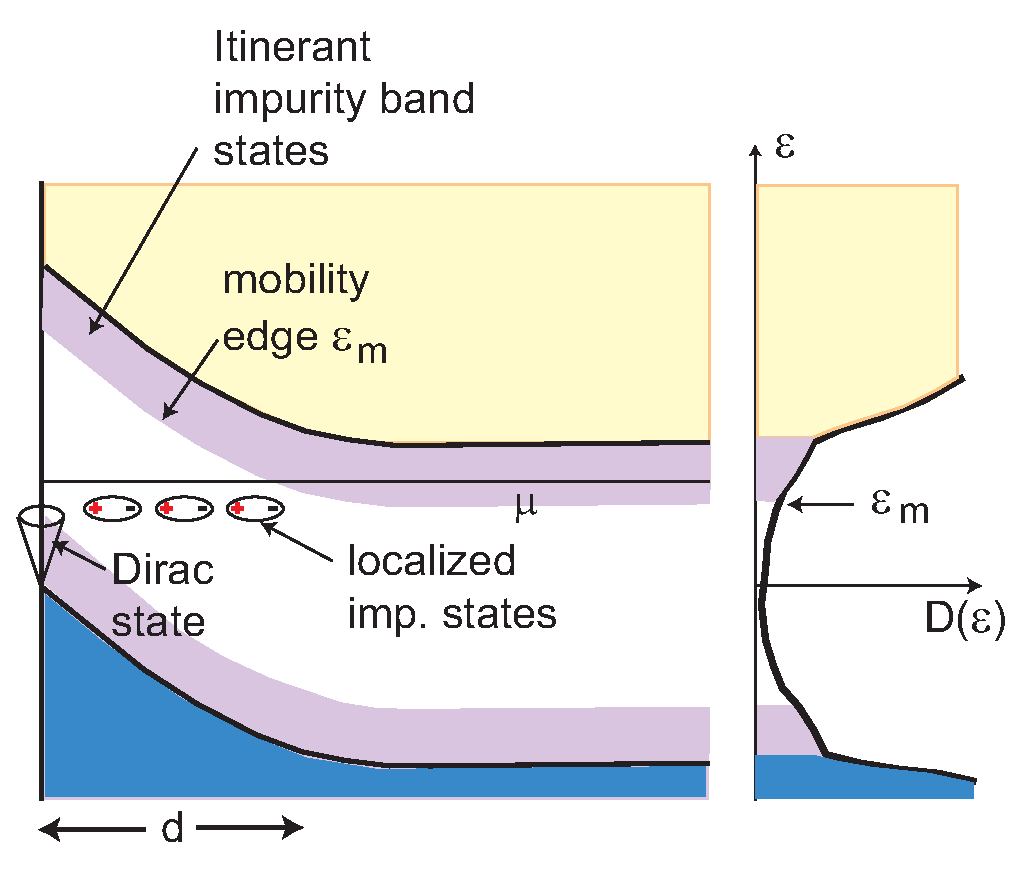
\includegraphics[width=0.65\linewidth]{ch-appendicies/figures/FigImpurityBand.eps}
\caption{\label{figimp}
Model for the impurity band states implied by the liquid-gating experiment. The density of states (DOS)
profile ${\cal D}(\varepsilon)$ across the bulk energy gap is sketched on the right. The impurity-band DOS tapers deep
into the gap, as suggested by STM experiments~\cite{Beidenkopf2011}. Impurity states lying above the mobility edge $\varepsilon_m$ (shaded)
are itinerant with mobility $\mu_b\sim$ 20 cm$^2$/Vs. States below $\varepsilon_m$ are strongly localized at 4 K. 
Near the surface (left sketch), $\varepsilon_m$ is lifted above 
$\mu$ within the depletion layer, substantially decreasing the bulk contribution to the observed $\sigma$ and $\sigma_H$. 
Localized states near the mobility edge (sketched as dipoles) contribute strongly to dielectric screening because of their 
enhanced polarizability.
}
  \end{center}
\end{figure} 


With reference to Fig. \ref{figGate}, the free-charge density profile $\rho(x)$ is comprised of 
4 delta functions $\delta(x)$ and an extended distribution over the depletion width $d$ (which we assume has a flat 
profile expressed by the step-function $\theta(x)$~\cite{Ashcroft}, as shown in Fig. \ref{figGate}(b). Setting the origin $x=0$ at the TI surface, we have
\begin{eqnarray}
\rho(x) &=& -\frac{Q}{A'}\delta(x+s) + \frac{Q}{A'}\delta(x+s-a) -\frac{Q}{A}\delta(x+a) \notag\\
 				&& +\sigma_s \delta(x) + N_ded\,[\theta(x)-\theta(x-d)],
\label{rho}
\end{eqnarray}
where $\sigma_s$ is the surface charge density at the exposed crystal face,
and $N_d$ is the density of ionized donor impurities within the depletion width $d$ (we take $e>0$). The electrostatic potential $\varphi(x)$ is derived from the Poisson equation
\be
-\varepsilon(x) \frac{\partial^2\varphi}{\partial x^2} = \frac{\rho(x)}{\epsilon_0},
\label{phi}
\ee
with $\epsilon_0$ the vacuum permittivity. The dielectric function $\varepsilon(x) = \epsilon_s$ inside the TI ($x>0$). Within the ionic liquid,
$\varepsilon(x) = \epsilon_{liq}$.

Integration of Eq. \ref{phi} gives the profile of $\varphi(x)$ sketched in Fig. \ref{figGate}b. We wish to relate the
charge density $Q/A$ to $\sigma_s$ and $d$.
Setting $\varphi$ and $\partial\varphi/\partial x$ to 0 
deep in the bulk ($x>d$), we have for the $E$-field just to the right of $x = 0$
\be
E(0^+) = -\left(\frac{\partial\varphi}{\partial x}\right)_{0+} = - \frac{N_ded}{\epsilon_0\epsilon_s}.
\label{E0}
\ee
In the flat-profile approximation for $\rho(x)$, Eq. \ref{phi} gives the parabolic variation of $\varphi(x)$ 
\be
\varphi(x) = -\frac{N_de}{2\epsilon_0\epsilon_s}(x-d)^2   \quad (x>0).
\label{varphi}
\ee

Next, we integrate Eq. \ref{phi} between the limits $x = 0^{\pm}$ (bracketing $x =0$) to get
\be
\epsilon_s E(0^+) - E(0^-) = \sigma_s/\epsilon_0.
\label{EE}
\ee
Together, Eqs. \ref{E0} and \ref{EE} give for the $E$-field just to the left of the surface
\be
E(0^-) = -(\sigma_s + N_ded)/\epsilon_0.
\label{E0-}
\ee
This strong $E$-field emanating from the anion charge $-Q$ is only partially screened by the surface charge $\sigma_s$. The remaining
$E$ penetrates a distance $d$ into the bulk until screened by enough ionized donor charge. The lattice polarizability,
expressed by the bulk dielectric constant $\epsilon_s$,
also contributes to the screening. (It is helpful to represent the dielectric screening, alternatively, as a 
bound-surface charge density $\sigma_b = -\epsilon_0(\epsilon_s-1)E(0^+)$ at $x$ = 0. However, this bound charge
should not be included in $\rho(x)$).


Finally, identifying $E(0^-)$ with the $E$-field within the molecular layer, $-Q/A\epsilon_0$, we arrive at the equation
\be
\frac{Q}{A} = N_ded + \sigma_s.
\label{Q}
\ee
We note that Eq. \ref{Q} is independent of $\epsilon_s$.
The charge $Q$ induced by the anions is partitioned between two charge reservoirs which see the same potential drop $V_s = \varphi(0)$ relative to the 
ground at $x=+\infty$. Hence, as shown in Fig. \ref{figGate}c, we regard the two charge reservoirs 
as two capacitors in parallel, namely the 
quantum capacitance~\cite{Luryi}
\be
C_q = \frac{\sigma_s}{\varphi(0)} = e^2\frac{dn_s}{d\mu},
\label{Cq}
\ee 
and the depletion-layer capacitance 
\be
C_d = N_dedA/\varphi(0).
\label{Cd}
\ee
Whereas in graphene, the quantum capacitance is readily resolved,
here it is shunted by the large $C_d$.

The parallel combination $C_q+C_d$ is in series with the ionic-liquid capacitor $C_0$ (the series combination of the cation and anion capacitors). The
voltage drop across $C_0$ is $V_G-V_s$.


\vspace{3mm}
%\noindent

We discuss a scenario in which a strongly enhanced electronic polarizability arises 
within the depletion layer. Figure \ref{figimp} is a sketch of the band bending near the surface. 
As shown, the chemical potential $\mu$ in the bulk lies just below the bottom of the conduction band.
The right panel plots the density of states ${\cal D}(\varepsilon)$ in a cut in the bulk.
The impurity band is comprised of ``tails'' of ${\cal D}(\varepsilon)$ which taper downwards (upwards) from the
conduction band (valence band)~\cite{Beidenkopf2011}. At 4 K, the mobility edge
$\varepsilon_m$ sharply divides states that are itinerant (closer to the gap edge) from 
the states that are localized. Electrons in the itinerant states diffuse with the observed mobility $\mu_b\sim$ 20 cm$^2$/Vs. 
In an $E$-field strong enough to cause band bending, 
$\varepsilon_m$ is lifted above $\mu$ within the depletion region of width $d$. Occupied states within this 
region are strongly localized, so they do not contribute to the observed conductivity or Hall effect. 
However, because the localization length $\xi_{loc}$ diverges as $\varepsilon\to \varepsilon_m$ from below, 
the localized states have a greatly enhanced electronic polarizability. 
The electronic component of the dielectric screening parameter will be much
larger than that from the lattice polarizability.
